\section{Закон сохранения импульса}

\introProblems

\begin{ex} %Сив187
С какой скоростью $v$ после горизонтального выстрела из винтовки стал двигаться стрелок, стоящий на весьма гладком льду? Масса стрелка с винтовкой и снаряжением составляет 70 кг, а масса пули 10 г и ее начальная скорость 700 м/с.
\begin{ans}
$v=10$ см/с.
\end{ans}
\end{ex}

\begin{ex} %Сив188
Определить силу, с которой винтовка действует на плечо стрелка при выстреле, если считать, что со стороны винтовки действует постоянная сила и смещает плечо стрелка на $S = 1,5$ см, а пуля покидает ствол мгновенно. Масса винтовки 5 кг, масса пули 10 г, и скорость ее при вылете равна $v = 500$ м/с.
\begin{ans}
$F = \frac{m^2 v^2}{2SM}$
\end{ans}
\end{ex}

\begin{ex} %Сив191
Три лодки одинаковой массы $m$ идут в кильватер (друг за другом) с одинаковой скоростью $v$. Из средней лодки одновременно в переднюю и заднюю лодки бросают со скоростью $u$ относительно лодки грузы массы $m_1$. Каковы будут скорости лодок после переброски грузов?
\begin{ans}
$v_1 = \frac{m_1(v+u)+mv}{m+m_1}$, $v_2 = v$, $v_3 = \frac{m_1(v-u)+mv}{m+m_1}$.
\end{ans}
\end{ex}

\begin{ex} %Сив194
В шар массы $m_1$, движущийся со скоростью $v_1$, ударяется другой шар массы $m_2$, догоняющий первый в том же направлении со скоростью $v_2$. Считая удар абсолютно неупругим, найти скорости шаров после удара и их кинетическую энергию.
\begin{ans}
$v = \frac{m_1v_1 + m_2v_2}{m_1+m_2}$, $K = \frac{(m_1v_1+m_2v_2)^2}{2(m_1+m_2)}$.
\end{ans}
\end{ex}

\begin{ex} %Сив190
Снаряд разрывается в верхней точке траектории на высоте $h = 19,6$ м на две одинаковые части. Через секунду после взрыва одна часть падает на Землю под тем местом, где произошел взрыв. На каком расстоянии $S_2$ от места выстрела упадет вторая часть снаряда, если первая упала на расстоянии $S_1 = 1000$ м от места выстрела? Сил сопротивления воздуха при решении задачи не учитывать.
\begin{ans}
$S_2 = 5$ км.
\end{ans}
\end{ex}

\qualProblems

\begin{ex}
Яблоко падает с дерева. Какое из следующих утверждений не объясняет, почему при этом яблоко набирает скорость?
\begin{itemize}
\item Полный импульс системы Земля-яблоко сохраняется.
\item На яблоко действует гравитационная сила, направленная к центру Земли.
\item Сила гравитации совершает положительную работу при падении яблока.
\item Яблоко теряет потенциальную энергию при падении.
\end{itemize}
\end{ex}

\begin{ex}
Почему стальной шарик хорошо отскакивает от мраморной плиты и хуже от асфальта?
\end{ex}

\begin{ex}
Почему пуля, вылетевшая из ружья, не может открыть дверь, но пробивает в ней отверстие? Почему давлением пальца  дверь открыть легко, но проделать отверстие невозможно?
\end{ex}

\begin{ex}
Каким молотком — легким или тяжелым — должен пользоваться скульптор для работы с долотом? Каким молотком лучше забивать гвозди? Когда упругий удар (с отдачей молотка) выгоднее неупругого? Тяжелее или легче сваи должен быть копёр для забивания свай?
\end{ex}

\begin{ex}
Представьте, что Вы ловите бейсбольный мяч, а затем некто предлагает Вам поймать мяч для боулинга либо летящий с таким же импульсом, либо летящей с такой же энергией. Что Вы выберете и почему?
\end{ex}

\begin{ex}
Как известно, движение центра масс тела может изменяться только под действием приложенной к телу внешней силы, однако вы можете проехать через комнату на стуле, не касаясь пола ногами. Если ваши судорожные движения на стуле связаны с внутренними силами, то чем же обусловлена внешняя сила?
\end{ex}

\begin{ex}
Как будет двигаться изображенная на рисунке тележка после открывания крана? Трением колес о плоскость пренебречь.

\begin{figure}[h]
\centering
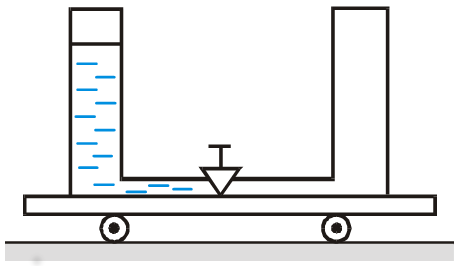
\includegraphics[width=0.5\textwidth]{U-vessel.png}
\caption{}
\label{U-vessel}
\end{figure}
\end{ex}

\simpleProblems

\begin{ex} %Сив199
С какой скоростью $v$ должен лететь снаряд массы $m$ = 10 кг, чтобы при ударе о судно массы $М$ = 100 т последнее получило скорость $v_1$ = 0,1 м/с? Удар считать неупругим.
\begin{ans}
1 км/c.
\end{ans}
\end{ex}

\begin{ex} %Чертов2.12
Шарик  массой 100 г упал с высоты 2.5 м на горизонтальную плиту, масса которой много больше массы шарика и отскочил от нее вверх. Считая удар абсолютно упругим, определите импульс, полученный плитой.
\begin{ans}
1.4 кгм/c.
\end{ans}
\end{ex}

\begin{ex} %Чертов2.34
Шар массой 10 кг, движущийся со скоростью 4 м/с, сталкивается с шаром массой 4 кг, скорость которого равна 12 м/c. Считая удар приямым, неупругим, найти скорость шаров после удара в двух случаях: 1) малый шар нагоняет большой шар, движущийся в том же направлении; 2) шары движутся навстречу друг другу.
\begin{ans}
1) 6.3 м/с; 2) 0.57 м/с.
\end{ans}
\end{ex}


\begin{ex} %Сив200
Ледокол, ударяясь о льдину массы $М$, отбрасывает ее, сообщив ей скорость $v$ [м/с]. Положим, что давление ледокола на льдину нарастает равномерно во времени при сближении ледокола со льдиной и также равномерно убывает, когда они расходятся. Найти при этих условиях максимальную силу давления льдины на борт корабля, если удар продолжался $\tau$ [с].
\begin{ans}
$F = 2Mv/\tau$.
\end{ans}
\end{ex}

\begin{ex} %Сив201
В одном изобретении предлагается на ходу наполнять платформы поезда углем, падающим вертикально на платформу из соответствующим образом устроенного бункера. Какова должна быть приложенная к платформе сила тяги, если на нее погружают 10 т угля за 2 с, и за это время она проходит равномерно 10 м? Трением при движении платформы можно пренебречь.
\begin{ans}
$F = \Delta m v/ \Delta t$.
\end{ans}
\end{ex}

\begin{ex} %Сив193
Две лодки идут навстречу параллельным курсом. Когда лодки находятся друг против друга, с каждой лодки во встречную перебрасывается мешок массой в 50 кг, в результате чего первая лодка останавливается, а вторая идет со скоростью 8,5 м/с в прежнем направлении. Каковы были скорости лодок до обмена мешками, если массы лодок с грузом равны 500 кг и 1 т соответственно?
\begin{ans}
9 м/с и 1 м/с.
\end{ans}
\end{ex}

\begin{ex} %Сив233
Лодка массы $M$ с находящимся в ней человеком массы $m$ неподвижно стоит на спокойной воде. Человек начинает идти вдоль по лодке со скоростью $\vec{u}$ и относительно лодки. С какой скоростью $\vec{w}$ будет двигаться человек относительно воды? С какой скоростью $\vec{v}$ будет при этом двигаться лодка относительно воды? Сопротивление воды движению лодки не учитывать.
\begin{ans}
$\vec{w} = \frac{M\vec{u}}{M+m}$, $\vec{v} = -\frac{m\vec{u}}{M+m}$.
\end{ans}
\end{ex}

\begin{ex} %Сив234
Пусть человек прошел вдоль по лодке, описанной в предыдущей задаче, его перемещение составило $\vec{l}$. Каковы будут при этом смещения лодки $\vec{S_1}$ и человека $\vec{S_2}$ относительно воды?
\begin{ans}
$\vec{S_1} = -\frac{m\vec{l}}{M+m}$, $\vec{S_2} = \frac{M\vec{l}}{M+m}$.
\end{ans}
\end{ex}

\complexProblems

\begin{ex} %Иродов1.129
В момент, когда скорость падающего тела составила $v_0 = 4,0$ м/с, оно разорвалось на три одинаковых осколка. Два осколка разлетелись в горизонтальной плоскости под прямым углом друг к другу со скоростью $v = 5,0$ м/с каждый. Найти скорость третьего осколка сразу после разрыва.
\begin{ans}
$u = \sqrt{9v_{1}^2 + 2v^2} = 14$ м/с.
\end{ans}
\end{ex}

\begin{ex} %Иродов1.132
Цепочка массы $m = 1,00$ кг и длины $l = 1,40$ м висит на нити, касаясь поверхности стола своим нижним концом. После пережигания нити цепочка упала на стол. Найти полный импульс, который она передала столу.
\begin{ans}
$p = (2m/3)\sqrt{2gl} = 3,5$ кг$\cdot$м/c.
\end{ans}
\end{ex}

\begin{ex} %МФТИ3.5
С какой силой пожарный должен удерживать пожарный шланг, вода из которого выбрасывается в виде потока мелких капель в количестве $Q = 10$ кг/с и может добивать до высоты $h = 10$ м? Оцените, какая сила будет действовать на стену, если на нее направить струю из этого шланга под углом $45^{\circ}$ (оценку провести в двух предельных случаях -- для упругого и для неупругого соударения капель со стенкой).
\begin{ans}
$F_1 = Q\sqrt{2gh} \approx 140$ Н, $F_2 = \sqrt{2} F_1 \approx 200$ Н, $F_3 = F_1/\sqrt{2} \approx 100$ Н. 
\end{ans}
\end{ex}

\clearpage